%%Target for future reference:
%http://www.journals.elsevier.com/environmental-modelling-and-software/

%Latex Configuration
%Init document class
\documentclass[11pt]{article}
\usepackage[margin=1.25in]{geometry}        

%Package for Authors on Title Page
\usepackage{authblk}

%Double Spacing Package
\usepackage{setspace}

%Biblatex Init
\usepackage[backend=bibtex, style=authoryear, citestyle=authoryear]{biblatex}
\bibliography{geoSimex}

%Figures Init
\usepackage{graphicx}
\graphicspath{ {images/} }

%Enable footnotes in tables
\usepackage{tablefootnote}

%Enable the \text{} command for use in equations
\usepackage{amsmath}

% For importing results
\usepackage{import}

% For formatting simulation results table:
\usepackage{dcolumn}
\usepackage{lscape}
\newcolumntype{M}[1]{>{\centering\arraybackslash}m{#1}}

\newcommand{\specialcell}[2][c]{%
  \begin{tabular}[#1]{@{}l@{}}#2\end{tabular}} 

%Authors and Affiliations
\author[1]{Daniel Runfola}
\author[1]{Rob Marty}
\author[1]{Seth Goodman}
\author[1]{Michael LeFew}
\affil[1]{Institute for the Theory and Practice of International Relations, AidData, The College of William and Mary}
\renewcommand\Authands{ and }

%Title
\title{Introducing geoSIMEX: A Generalized Approach To Modeling Spatial Imprecision}

%-------------------------------------
%-------------------------------------
%Analysis
%-------------------------------------
%-------------------------------------


\usepackage{Sweave}
\begin{document}
\Sconcordance{concordance:master.tex:master.Rnw:%
1 21 1 1 5 2 1 1 0 9 1}
\Sconcordance{concordance:master.tex:./title.Rnw:ofs 35:%
1 11 1}
\Sconcordance{concordance:master.tex:master.Rnw:ofs 47:%
40 5 1}
\Sconcordance{concordance:master.tex:./abstract.Rnw:ofs 53:%
1 10 1}
\Sconcordance{concordance:master.tex:master.Rnw:ofs 64:%
47 2 1}
\Sconcordance{concordance:master.tex:./introduction.Rnw:ofs 67:%
1 58 1}
\Sconcordance{concordance:master.tex:master.Rnw:ofs 126:%
51 2 1}
\Sconcordance{concordance:master.tex:./dataMethods.Rnw:ofs 129:%
1 183 1}
\Sconcordance{concordance:master.tex:master.Rnw:ofs 313:%
55 2 1}
\Sconcordance{concordance:master.tex:./results.Rnw:ofs 316:%
1 20 1}
\Sconcordance{concordance:master.tex:master.Rnw:ofs 337:%
59 2 1}
\Sconcordance{concordance:master.tex:./discussion.Rnw:ofs 340:%
1 24 1}
\Sconcordance{concordance:master.tex:master.Rnw:ofs 365:%
63 2 1}
\Sconcordance{concordance:master.tex:./conclusion.Rnw:ofs 368:%
1 14 1}
\Sconcordance{concordance:master.tex:master.Rnw:ofs 383:%
67 2 1}
\Sconcordance{concordance:master.tex:./tables.Rnw:ofs 386:%
1 52 1}
\Sconcordance{concordance:master.tex:master.Rnw:ofs 439:%
71 2 1}
\Sconcordance{concordance:master.tex:./figures.Rnw:ofs 442:%
1 12 1 1 5 7 1}
\Sconcordance{concordance:master.tex:master.Rnw:ofs 463:%
75 2 1}
\Sconcordance{concordance:master.tex:./acknowledgements.Rnw:ofs 466:%
1 1 1}
\Sconcordance{concordance:master.tex:master.Rnw:ofs 468:%
79 5 1}


%-------------------------------------
%-------------------------------------
%Paper Sections 
%-------------------------------------
%-------------------------------------

%Title Page (title.Rnw)
\maketitle 
\begin{flushleft}
\textbf{Corresponding Author}:\\
Dr. Daniel Runfola\\
Institute for the Theory and Practice of International Relations, \emph{AidData}\\
427 Scotland Street, Williamsburg, VA 23185\\
Email: dsmillerrunfol@wm.edu
Telephone: 508.316.9109
Fax: 757.221.4650
\end{flushleft}


\newpage

%Toggle spacing for document
\doublespacing

%Abstract (abstract.Rnw)
\section{Abstract}
Spatial imprecision exists in nearly all spatial information - from census data to satellite information, the exact geographic location to which a measurement can be attributed is rarely known.
Following this, there is a large and growing set of literature examining how different classes of models can integrate information on spatial imprecision in order to more accurately reflect available data.
Here, we present a flexible approach - geoSIMEX - which can provide parameter and error estimates for both linear and non-linear models while adjusting for spatial imprecision.
Further, this approach can provide an estimate of the potential value of additional spatial information by distinguishing between traditional model error and additional errors introduced by imprecision.
We illustrate this approach through a case study leveraging a novel, publically available dataset recording the location of Chinese aid in Africa at varying levels of precision.
Using a difference-in-difference model, we integrate this information with satellite derived data on vegetation (NDVI) and a number of other spatially explicit covariates to examine if there is evidence Chinese aid has caused an increase or decrease in vegetation.
Following commonly employed procedures which do not incorporate spatial imprecision, we found that Chinese Aid had a negative impact on vegetation; once spatial imprecision was incorporated into our estimates through the geoSIMEX procedure no evidence of impact was found.
We use these findings to argue for the importance of incorporating spatial imprecision into analyses, and introduce new software in the R programming language to enable similar analyses for other purposes.

\textbf{Keywords}: SIMEX, Spatial Uncertainty, Spatial Data Integration, Simulation, Ecological Fallacy\\
\newpage

%Introduction
\section{Introduction}
The lack of exact geographic information on where measurements are obtained presents a barrier to research.
This has become increasingly evident as more scholars integrate geographic data from multiple sources - for example, census, satellite, and GPS sources - to try and establish causal or predictive relationships (c.f., EXAMPLES).
Many scholars have engaged in research seeking to integrate information on the precision of geographic data to improve the accuracy of modeling efforts, variably referred to as spatial (im)precision (CITE), spatial uncertainty (CITE), and spatial allocation (CITE).
This paper presents a generalizeable approach to integrating information on the precision of geographic data into both linear and non-linear models - geoSIMEX.
We illustrate the capability of geoSIMEX to provide more accurate parameter estimates than traditional approaches through a simulation framework. 
Using a novel dataset, we then apply both tradional models and a geoSIMEX model to examine the causal impact of Chinese Aid on vegetation in Africa.
We use this case study to illustrate the importance of including information on spatial imprecision into analyses.
Finally, we provide all data and an accompanying R package to users seeking to perform similar styles of analysis.

\subsection{Literature Review}
% (dont include SIMEX here, just general lit on spatial uncertainty..  3 paragraphs.)

The literature has shown that uncertainty in the locations of where measurements were taken can produce biased estimates in empirical analyses.\cite{perez-heydrich_guidelines_2013,rettie_overcoming_1999} For example, Perez-Heydrich et al. show that regression coefficients will be biased when using raster data in conjunction with point data, where the true locations of the point data are only known to exist within some 5-10km radii of the measured location.\cite{perez-heydrich_guidelines_2013} One recommended solution is to take average raster values within a buffer encompassing where the point could have fallen, instead of the single raster value associated with the point.\cite{perez-heydrich_guidelines_2013, rettie_overcoming_1999}
\par
Another practice to address spatial uncertainty is to aggregate to some higher spatial scale where there is no spatial uncertainty.\cite{perez-heydrich_guidelines_2013} However, aggregating to a higher spatial scales can introduce bias. A large body of literature shows that analyzing data at different levels of aggregation can produce different regression coefficients and correlation coefficients.\cite{clark_effects_1976, selvin_durkheims_1958, gotway_combining_2002, gehlke_certain_1934, cramer_efficient_1964} Estimates from aggregate data are invalid for disaggregate data due to different magnitude of correlations and regression coefficients. For example, a seminal study by Robinson illustrates this point. Using data from the 1930 US census, Robinson found a negative correlation between the proportion of immigrants in a state and average literacy levels, but a positive correlation between being an immigrant and literacy level.\cite{robinson_ecological_2009} A number of techniques have been proposed to address aggregation bias. Approaches focus on dis-aggregating data to finer scales; however, these involve using covariats to help predict the variable of interest.\cite{gotway_combining_2002, zhu_combined_2004} 

% ** Other Studies Incorporating Spatial Uncertainty **

% \item Krigging techniques have been developed that account for error in the spatial locations of where measurements are recorded.\cite{CressieKornak:2003}

\subsection{(geo)SIMEX}
%1-2 paragraphs outlining the basic principles of SIMEX with cites and equations.
The simulation and extrapolation method (SIMEX) provides one solution to address measurement error in covariates (CITE). SIMEX exploits the fact that greater measurement error will lead to greater bias following a two step process. First, SIMEX simulates additional measurement error to establish a relation between measurement error and covariate bias. Second, it uses the relation between error and bias to extrapolate to a point with zero measurement error, thus providing an estimate of the unbiased coefficient.
\par
SIMEX simulates error using the following equation:
\begin{equation}
X(\lambda) = X + \sqrt{\lambda}U
\end{equation}
where X is the measured covariate, U is the variance of the measurement error and $\lambda$ is a parameter that simulates additional measurement error. $\lambda=0$ corresponds to the original amount of measurement error in the measured covariate, X. SIMEX uses increasing values of $\lambda$ (e.g., 0.5, 1, 1.5, and 2) to estimate models with simulated amounts of additional measurement error. SIMEX then estimates a trend between $\lambda$ and the coefficient on X, and uses the trend to extrapolate back to $\lambda = -1$ (point of no measurement error).
\par
In geoSIMEX, we take this approach and modify $\lambda$ to capture the degree of spatial imprecision in a given dataset, relative to the maximum amount of imprecision that could be observed.
The practical need for a geographic version of SIMEX can be demonstrated through a hypothetical example, in which a researcher seeks to measure the degree to which the amount of precipitation across 200 fields can explain the number of apples grown in each field.
These hypothetical researchers measure precipitation in each of 200 fields using satellite imagery, and counts each of the apples by hand.
In the simplest form, these researchers then use these measurements to model the relationship between rainfall and apples following:
\begin{equation}\label{eq:precip}
\text{CountOfApples} = \beta_{0} + \theta * \text{Rainfall} + \sum{\beta_{j} * X_{j}} + \epsilon
\end{equation}
\noindent in which $\beta_{j}$ and $X_{j}$ represent vectors of parameter estimates and controls, respectively. 
In this equation, a common goal would be to estimate $\theta$ with a high degree of accuracy, as this parameter helps to explain the degree to which precipitation impacted the count of apples.
\par
In this example, if each field was a perfect square of the same resolution as the satellite imagery (and had perfect overlap), then the measurements of rainfall would have no measurement error due to imprecision.
In practice, this rarely is the case, and thus the parameter $\theta$ can be biased due to imprecision in measurements.
Consider, for example, the worst case of imprecision in which a coarse reolution satellite sensor provides only one measurement of rainfall for every crop.
A responsible researcher seeking to use this data might leverage a model averaging framework to overcome concerns of the ecological fallacy - i.e., randomly distributing rainfall to each crop, fitting equation \ref{eq:precip}, and repeating this hundreds of times to estimate the range of possible coefficients that could be observed given the available data.
However, in cases of complete spatial imprecision, these estimates will be heavily biased towards 0.
This has two implications - first, the mean estimated coefficient will likely under-estimate the true coefficient, and second the distribution of possible coefficients (i.e., at a 95\% confidence level) will be centered at this biased coefficient.  
This suggests that not only can mean estimates be incorrect, but under cases of spatial imprecision statements regarding the significance of variables can also be biased.
\par
While it is rare that satellite measurements perfectly line up with units of analysis, it is also rare that researchers only have one measurement for all units of analysis.
More reasonably, researchers commonly have a mixture - i.e., satellite imagery that may cover portions of some crops but not others, leading to variable imprecision across the study area.
geoSIMEX takes advantage of the known level of precision in the data available ot the research (which we define as $\lambda$), and intentionally adds imprecision to establish the relationship between additional imprecision and coefficient bias.
The geoSIMEX procedure then uses this relationship to back-extrapolate to an unbiased coefficient estimate, i.e. the value at $\lambda$ = 0.
Finally, we employ a bootstrapping procedure to estimate the additional variance attributable to spatial imprecision.





\newpage

%Data and Methods
\section{Data and Methods}
This study leverages a novel dataset on the location of Chinese international aid in Africa available at varying levels of precision (i.e., the exact location of each aid project is not always known).  
It integrates this information with a variety of other ancillary datasets, including the NASA Long Term Data Record (LTDR) to examine the causal impact of Chinese aid on vegetation.  
Employing geoSIMEX, we use this case study to illustrate the importance of incorporating information on spatial imprecision into analyses.
\subsection{Data}
To conduct this analysis, a new dataset on the location of Chinese aid is derived through a methodology designed to Track Underreported Financial Flows (the TUFF methodology).  
This dataset is merged with a number of existing datasets, retrieved from publically available sources as described below.

\subsubsection{Study Area and Scope}
China has increasingly taken a larger role near home in providing aid to developing countries.
In this analysis, we examine the impact of Chinese aid in southeast asia, explicitly focusing on Cambodia, Laos, Myanmar, Thailand and Vietman.
Using the Global Administrative Areas (GADM; CITE) database, we aggregate Chinese aid, covariate and outcome information to the second-level administrative units within each country (see figure \ref{fig:studyarea}).

%210 = Transport and Storage


\subsubsection{Aid Information - Tracking Underreported Financial Flows (TUFF)}
Unlike many donors, China does not publically report the international aid they send (CITE).
(Placeholder for TUFF details)
Due to the considerable spatial imprecision generated by the TUFF process, we use this variable as an illustrative case of how the geoSIMEX procedure can be used to provide better estimates than traditional approaches.

% Precision Codes
% PC1 = 90 project locations
% PC2 = 12 project locations
% PC3 = 63 project locations
% PC4 = 34 project locations
% PC6 = 18 project locations
% PC8 = 5 project locations

%220 = Communications
%230 = Energy Generation and Supply
%320 = Industry, Mining, Construction

%USD-2011 deflation

% The resulting dataset includes 65 discrete projects allocated across 222 project locations, totaling in $7,729,666,290 committed.


\subsubsection{Ancillary Datasets}
Covariate data is collected from a variety of sources, summarized in table \ref{data_source_table}.
Our outcome measure - fluctuation in NDVI - is derived from the NASA Long Term Data Record (LTDR) dataset.
While relatively coarse resolution, this dataset represents the longest consistent record of NDVI available at the global scale.
To facilitate our difference-in-difference modeling efforts, we further select a number of covariates we believe could also impact shifts in NDVI (other than Chinese aid).
These include:
\begin{enumerate}
\item{Long-term climate data from the University of Delaware, providing precipitation and temperature data at a monthly time-step for the full data record, which is permuted to produce yearly mean, minimum, and maximum values for each project location.}
\item{Population Data is retrieved from CIESIN at Columbia University, specifically leveraging the Gridded Population of the World (GPW) data record.}
\item{Slope and Elevation data are derived from the Shuttle Radar Topography Mission (SRTM).}
\item{Distance to rivers is calculated based on the USGS Hydrosheds database.}
\item{Distance to roads is calculated based on the Global Roads Open Access Dataset (gRoads), which represents roads circa 2010, though the actual date of datasets is highly variable by country.}
\item{Urban travel time, calculated by the European Commission Joint Research Centre.}
\item{Nighttime Lights are retrieved from the NOAA Earth Observation Group, calculated from the Department of Defense Defense Meteorological Satellite Program (DMSP).  Lights values are temporally intercalibrated following the procedure outlined in \cite{weng_global_2014}}
\end{enumerate}
Each of these datasets are processed and aggregated according to their average values within each district included in this analysis.  
Further, the size of districts are controlled for to mitigate the challenge of variably-sized districts across the study area.
In cases where covariates were measured at a resolution coarser than the unit of observation, the relative area of overlap was used to generate a weighted mean.
Further information on this decision can be found in the discussion.

\subsection{Methods}
Two different modeling processes are followed.  First, we use a monte carlo simulation procedure to illustrate the relative accuracy of geoSIMEX as contrasted to other procedures.  Second, we apply geoSIMEX to the case of Chinese Aid in Africa.

\subsubsection{geoSIMEX}
We employ geoSIMEX to identify the impact of Chinese Aid on vegetation, measured by a satellite-derived measure of NDVI.
We specifically seek to adjust for bias in the relative spatial imprecision of where Chinese Aid is located - imprecision largely due to the lack of formal information published by the Chinese government.
We describe this process through an illustrative example, in which we attempt to solve the following simplified equation:
\begin{equation}
NDVI = \theta * \text{Chinese aid} + \epsilon
\label{eqn:ndvi_aid}
\end{equation}
where, for the sake of example, Chinese aid is defined to be causally and positively related to a measure of NDVI by a one-to-one relation (e.g., $\theta$ = 1), and $\epsilon$ is a random error term. 
Aid is measured with spatial imprecision, and through using geoSIMEX we account for the spatial uncertainty to accurately estimate the model coefficient, $\theta$. 
\par
In figure \ref{fig:nepal_ex}, we present a hypothetical country with sixteen districts for which we seek to solve equation \ref{eqn:ndvi_aid}. 
Four of these sixteen units of analysis, districts 5,6,7, and 8 are distinguished on the map. 
Within this study area, a hypothetical data set contains three geocoded Chinese aid project locations of various levels of spatial precision, projects A, B, and C. 
Project A is assigned a coordinate pair in District 5 and had strong documentation, resulting
in precise geographic information (i.e. an exact latitude and longitude). 
Due to weaker project documentation, location B has a precision level indicating that it was allocated anywhere in the region that includes districts 5,6,7, and 8. 
Project C has very uncertain spatial information, such that it may be anywhere in the country. 
The area (in square kilometers) of the unit of analysis in which each project location may have been allocated gives us the size of the project location’s area of coverage, which is summarized in table \ref{precision_example}.
Using the spatial overlap between each region of interest (the sixteen districts) and the area an international aid project might exist in, we calculate a probability that each district contains a given project:

\begin{equation}\label{eq:overlaps}
V_{t} = \sum_{S}^{s=1}U_{s}\left ( \frac{a_{st}}{\sum_{T}^{t=1}a_{st}} \right )
\end{equation}

\noindent This represents the "no information" case - i.e., probabilities are only based on geographic overlap, as opposed to integrating other factors which might mediate where aid is allocated.
This equation can be modified to incorporate more information on spatial location, thus allowing a researcher to trade off additional assumptions or information about factors that mediate spatial allocation in exchange for higher degrees of spatial precision (i.e., through dasymetric mapping approaches).
\par
We use these probabilities in a modified version of the SIMEX procedure, geoSIMEX.  
In traditional SIMEX, measurement error is captured through scaling an estimated distribution of errors.
In our context, greater spatial imprecision is reflected by increasing the area of coverage of a project, thus expanding the probability a project could be located in a wider set of units of analysis. 
geoSIMEX exploits the fact that greater spatial imprecision will bias results towards 0 - i.e., if all data was measured at the country scale and every district had an equal probability of receiving aid, any results found using districts as the unit of analysis would be the equivalent of random noise.
geoSIMEX (a) calculated the initial level of spatial imprecision in a given dataset, and then (b) simulates additional spatial imprecision to establish this relationship between spatial imprecision and covariate bias. 
Based on this relationship, it extrapolates to a point with zero spatial imprecision, thus providing an estimate of the unbiased coefficient.
\par

\textbf{The first step} of geoSIMEX is to calculate the initial level of spatial imprecision in the given dataset, defined by $\lambda$.
To reflect imprecision across a given set of international aid projects and a set of units of analysis (i.e., districts), we calculate (\begin{math}\lambda\end{math}) following:

\begin{equation}\label{lambda}
\lambda = \frac{\sum_{i}^{P}Area \ of \ Coverage_i}{\sum_{i}^{P}Total \ Possible \ Area \ of \ Coverage_i}
\end{equation}

\noindent where $i$ is an individual project out of $P$ total Chinese Aid projects. $Area \ of \ Coverage_i$ is project $i$'s known area of coverage defined by the available documentation - i.e., the geographic area across which a project could be located. 
$Total \ Possible \ Area \ of \ Coverage_i$ is the area of coverage of project $i$ under complete spatial imprecision - e.g., the geographic area of the study area.
\par
If the latitude and longitude of every aid project was known, $\lambda$ would resolve to 0---indicating zero spatial imprecision. 
If spatial data was only available for the entire study area (e.g., aid provided for general budget support without indication of where the project was allocated), $\lambda$ would resolve to 1---indicating 100\% spatial uncertainty. 
In practice, combinations of different levels of precision result in $lambda$ values between these two extremes, providing a single linear measurement of spatial imprecision.
\par
\textbf{The second step} involves estimating a naive model (which can be of variable functional forms; for illustration we use ordinary least squares regression), where imprecision in aid is ignored. 
For each unit of observation, the value of aid used for modeling is the expected value of aid calculated following the geographic overlap-based probabilities described in (EQUATION!!).
In figure \ref{fig:steps}, we provide an example of the geoSIMEX procedure is applied to a dataset with an initial $\lambda$ value of 0.4, indicating the set of data provided was of moderate spatial precision relative to the units of observation.
In this figure, the x-axis represents the $\lambda$ value (spatial imprecision) for a dataset, with higher values indicating more imprecision.
The y-axis represents the estimated value of $\theta$ in equation \ref{wealth_aid}.
In \ref{fig:steps}a, the orange line represents the 95\% confidence interval of the coefficient on aid in this naive model. 
The horizontal black line represents the true model coefficient ($\theta$ = 1), which the naive model fails to capture.
\par 
In \textbf{the third step}, additional imprecision is simulated by randomly decreasing the precision of observations (in this case, Chinese Aid projects). 
For example, a project that has a measurement with an exact latitude and longitude will randomly be assigned a lower level of precision - i.e., a county, state, or even the entire country. 
Using these new, reduced levels of precision a model is fit in an identical fashion to step 1, and the estimated $\theta$ parameter, standard errors of the model,ad $\lambda$ value for a given permutation are saved.
This process is repeated 10000 times. 
In figure \ref{fig:steps}b, the black points represent individual iterations, with the saved model coefficients (y axis) and their associated $\lambda$ (x axis) values. 
\par
\textbf{The fourth step} subdivides this set of iterations into three equally-sized bins based on the level of spatial uncertainty ($\lambda$) of the aid variable (e.g., if $\lambda$ values range from 0.4 to 1, coefficients are separated into bins of 0.4-0.6, 0.6-0.8, and 0.8-1). 
Average coefficient and $\lambda$ values are calculated within each bin, represented as red dots in figure \ref{fig:steps}c. 
A quadratic trend is fit on the resulting average coefficient and lambda values. 
The trend is then extrapolated back to $\lambda=0$, thus providing an estimate of $\theta$ with perfect spatial precision. 
In figure \ref{fig:steps}d, the red line represents the extrapolated trend, and the blue dot represents the extrapolated estimate of the coefficient on aid. 
\par 

\textbf{In the fifth step}, the variance and standard errors of these estimates are calculated. 
We employ a bootstrapping method to calculate the component of the standard error resulting from spatial imprecision. Here, a point from each bin is sampled, a quadratic trend is fit on the resulting values, and the trend is extrapolated back to $\lambda$ = 0. 
This process is repeated 10000 times (defined as $R$). 
In figure \ref{fig:steps}e, each blue line represents one extrapolated trend and $\lambda$ = 0 estimate. 
We use a variance equation originally developed to capture model selection uncertainty to seperately incorporate both original standard errors and the additional error from spatial imprecision (CITE Burnham and Anderson):

\begin{equation}\label{variance}
var(\hat{\bar{\beta}}) = \sum_i^R \frac{1}{R} \{ var(\hat{\beta_i}) + (\hat{\beta_i}-\hat{\bar{\beta_i}})^2 \}
\end{equation}

\noindent where $R$ is the number of extrapolated coefficients (in this example, 1000). 
$var(\hat{\beta_i})$ is the standard error of each extrapolated coefficient, calculated by fitting a quadratic trend on the standard error estimates from each bin extrapolating back to $\lambda=0$ and collecting the resulting standard error value. 
$(\hat{\beta_i}-\hat{\bar{\beta_i}})^2$ captures the component of the variance from spatial uncertainty, where each extrapolated coefficient estimate is subtracted by the mean of all extrapolated coefficient estimates.  

\subsubsection{Simulations}

We employ a monte carlo procedure to determine the accuracy of geoSIMEX compared to other approaches to handle spatial imprecission. The procedure generates data to model the relation between Chinese aid and NDVI according to equation \ref{eqn:ndvi_aid}. Each simulation procedes in the following 7 steps:

\begin{enumerate}
\item One of three hypothetical countries with different administrative heirarchices is generated: (1) a country with 60 subcounties, 30 counties, 10 districts, and 2 regions, (2) a country with 120 subcounties, 40 counties, 20 districts, and 5 regions, or (3) a country with 120 subcounties, 60 counties, 30 districts, and 10 regions. Each subcounty is randomly assigned a spatial area and a probability of recieving aid. 
\item 50 to 250 aid projects are randomly allocated to subcounties, according to the assigned probability of a subcounty receiving aid. 
\item NDVI is generating according to equation \ref{eqn:ndvi_aid}. Specifically, NDVI is defined as the number of aid projects plus random error.
%\item Equation \ref{eqn:ndvi_aid} is estimated using an OLS model to capture the relation between Chinese aid an NDVI without spatial imprecession.
\item Each aid project is given a code indicating the spatial precision that a researcher might see. Codes range from indicating the project fell within a sub-county (no spatial imprecision), to falling somewhere within a county, district, region, or the country. 
\item The expected value of aid is calculated for each subcounty. For projects with spatial imprecission, aid is disbursed to subcounties based on spatial area, with larger subcounties having a larger probability of recieivng aid. For example, consider a project where \$1 million was disbursed to either subcounty A (spatial area of 400km) or subcounty B (spatial area 100km). Because subcounty A is four times as large as subcounty B, subcounty A will be assigned four times as much aid from the project as subcounty B. Specifically, subcounty A will be assigned \$800,000 and subcounty B will be assigned \$200,000. Disbursing aid using spatial area assumes that each location (e.g., each sq. kilometer) within a country has an equal chance of receiving aid.
\item Equation \ref{eqn:ndvi_aid} is estimated using two naive models that do not incorporate spatial imprecision: the first uses the expected value of aid, and the second only includes aid projects with complete spatial preceision.
\item Equation \ref{eqn:ndvi_aid} is estimated using geoSIMEX and a model averaging approach. In the model averaging approach, subcounties are assigned a random probability of receiving aid and the expected value of aid is calculated according to that probability. 500 models are estimated, where the average coefficient is used with the standard error estimated using equation \ref{variance}.
\end{enumerate}

This process is repeated 100,000 times. 

\subsubsection{Chinese Aid in Africa}
In an illustrative case study of geoSIMEX, we examine the causal impact that Chinese aid distributed from 2005 to 2010 had on vegetation (measured using NDVI) in southeast asia.  
A difference-in-difference modeling strategy is followed, in which the average of NDVI before aid was allocated (pre-2004) is contrasted to the average of NDVI after aid was allocated (post-2011) for each of 351 districts:
\begin{equation}\label{eq:caseStudy}
Y_{i} = \beta_0 + \theta * Aid_{i} + \sum_{i=k}^{n}(\beta_{k} * X_{i})
\end{equation}
Where $Y_{i}$ is the difference in the average forest loss post-2011 and pre-2004 in district $i$; $Aid_{i}$ is the log of the aid commitments to each district; $X_{i}$ is a vector of control variables; $\beta_{k}$ is a vector of parameters for each beta covariate, and $\theta$ is the estimated impact of aid.
We calculate the initial lambda value for our dataset following \ref{lambda}, and simulate additional spatial imprecision by allocating aid to increasingly coarse units of administration.  
For example, aid which was known to be allocated to a district might be instead allocated to a state, and the bias this introduces is estimated through a re-calculated $\lambda$ each geoSIMEX iteration.
We further repeat this analysis using three alternative modeling approaches to contrast their outcomes to geoSIMEX: (1) an ordinary least squares model in which imprecision is ignored (representative of a traditional case of the ecological fallacy), (2) a linear model in which all coarse-resolution data is removed from the dataset, and (3) a Monte Carlo model averaging approach in which hundreds of equally-probable worlds are generated based on the initial dataset, and the average beta coefficient and standard errors are reported.\footnote{It should be noted there are many approaches to model averaging, including AIC weighting, that are not tested in this paper. It is possible some of these alternative approaches may outperform the Monte Carlo procedure presented here.}











\newpage

%Results
\section{Results}
\subsubsection{Simulations}

Table (NUM) shows results from the simulation analysis. Results are subset according to the spatial imprecession of the Chinese aid data. The naive model using the expected value of aid captures true coefficient about 50\% of the time within a 95\% confidence interval when there is low spatial uncertainty ($\lambda < 0.3$), and the ability for the model to capture the true coefficient declines as spatial imprecesion increases. The naive model using the subset of aid projects measured with complete spatial uncertainty captures the true coefficient 60\% to 70\% of the time depending on the level of spatial imprecesion in the data. The model averaging approach performs well under low levels of spatial imprecession; however, as spatial imprecession increases the ability for the model averaging approach to capture the true coefficient decreases. Under low levels of spatial imprecession the model averaging approach captures the true coefficient 85\% of the time, but under high levels of spatial imprecession the model captures the true coefficient 46\% of the time. 
\par
The geoSIMEX model outperforms the model averaging approach in its ability to capture the true coefficient at all levels of spatial imprecession. At low levels of spatial imprecession the geoSIMEX model captures the true coefficient 90\% of the time; however, it captures both the true relation and statistical significance 52\% of the time compared to 84\% of the time from using model averaging. Higher spatial imprecesion leads to larger standard errors in the geoSIMEX model, reflected by the percentage of time the geoSIMEX model captures the true relation and statistical significance declining as spatial imprecesion grows. At high levels of spatial imprecesion ($\lambda > 0.7$), the geoSIMEX model captures the true relation 100\% of the time; however, large standard errors results in it capturing the true relation and statistical significance 0\% of the time.   

\subsubsection{Chinese Aid in Southeast Asia}
We examine the model results from our analysis of the impact of Chinese Aid in southeast Asia to provide an illustrative example of how accounting for spatial imprecision can lead to substantively different conclusions than alternative modeling approaches.
Table \ref{seresults} summarizes these findings.
In (1) a linear model that ignores spatial imprecision (i.e., commits an ecological fallacy), (2) a linear model that omits imprecise spatial information, and (3) a Monte Carlo model averaging approach, findings suggest that Chinese Aid has contributed to deforestation (or, more explicitly, an increase in the reduction of NDVI).
However, when the spatial imprecision of the data is explicitly modeled (4), we find that insufficient evidence exists to determine if Chinese Aid has had a positive or negative impact on vegetations.
\par
Figure \ref{fig:geoSIMEX_plot} provides an illustration of the geoSIMEX results calculated in model 4.
In this figure, the y axis represents coefficient estimates for aid ($\theta$), and the x axis represents the amount of spatial imprecision in the data calculated following equation \ref{lambda}.
The red point and line at $\lambda$ = .22 represents the solution that would be found when constructing a model which ignores spatial imprecision (equivalent to model 1 in table \ref{serresults}), in which the point represents the coefficient estimate for aid ($\theta$), and the line represents the 95\% confidence interval.
By simulating additional error and back-extrapolating to $\lambda$ = 0, the geoSIMEX estimate for aid ($\theta$) can be observed in the blue point in line, which is equivalent to model 4 in table \ref{serresults}.
\par
Further, leveraging geoSIMEX we seperately estimate the contribution of (1) spatial imprecision and (2) unexplained model variance to the standard errors estimated for $\theta$.
In this example, we find that ...

\newpage

%Discussion
\section{Discussion}
Broadly, this paper is related to papers that seek to overcome issues related to the Ecological Fallacy - i.e., the fallacy of measuring data at a course resolution and applying it to units of a finer resolution.
By treating this "fallacy" as a source of explicit uncertainty in the modeling process, we argue that the use of relatively coarse resolution data not only can provide more insight into processes of interest, but that by ignoring coarse-scale information researchers may be commiting a seperate fallacy - that of ignoring "known unknowns".
This can be particularly troublesome in analyses which seek to establish causal relationships between variables, as bias that results from spatial imprecision can lead to incorrect statements of the statistical significance of such relationships.
\par
While geoSIMEX mitigates many issues related to spatial imprecision, it is not a silver bullet solution.
First and foremost, the ability of geoSIMEX to uncover the true coefficient is heavily influenced by the initial precision of the observed data.
If a researcher attempts to use data which has complete imprecision (i.e., $\lambda$ = 1), the results provided by geoSIMEX will be meaningless as no information is available from which a trend can be estimated.
As $\lambda$ approaches 0 (perfect precision relative to the units of observation), geoSIMEX will provide increasingly accurate estimates as it has an increased number of $\lambda$ units to derive data for - i.e., there are more variable simulations across observations of $\lambda$.
This feature of geoSIMEX is novel when compared to traditional SIMEX.
In the traditional SIMEX process, an infinite amount of error can be simulated in any given variable by increasing the width of the error distribution.
In geoSIMEX, the maximum amount of imprecision in the system is limited by the spatial configuration of the study area (i.e., the maxmium imprecision is observed when all measurements are taken at the scale of the entire study area).
\par
There are many directions for future work.
First, the process described here should be generalizeable to multiple dimensions of spatial imprecision - i.e., imprecision in multiple attributes of the data.
Such multidimensional approaches to SIMEX have been examined in other fields (CITE), but applying them to the case of geographic imprecision should help to overcome many issues surrounding data integration alluded to in this piece.
Second, the authors hypothesize that the SIMEX procedure could be applied not only to cases of imprecision in observed variables (the ecological fallacy), but may also provide a solution to the ever-present concern of arbitrary units of observation (the modifiable area unit problem, or MAUP).
By treating the boundaries of units of observation as a unique cause of spatial imprecision (i.e., the exact - or correct - boundaries may not be known), geoSIMEX could be modified to provide estimates unbiased by covariates or boundary selection.
However, both computational and methodological barriers remain to this solution.
Finally, in non-hierarchical datasets the application of geoSIMEX is currently not feasible due to a lack of a relevant "weights" matrix to establish how data should be permuted at higher levels of $\lambda$.
For example, in a raster dataset coarsening data can be done simply by aggregating nearby grid cells; conversely, if one sought to examine the impact of global international aid on non-contigious protected areas, it is unclear how imprecisions should be introduced into the system.
\par
geoSIMEX has a secondary benefits in the ability to seperately identify traditional model errors and errors introduced due to spatial imprecision (see eq. \ref{variance}).
By breaking these sources of error out, one could provide estimates of how much value additional information on spatial imprecision could provide to a given analysis.
This information could be useful in the justification of more precise approaches to spatial measurement.
\newpage

%Conclusion
\section{Conclusion}
In this piece, we introduce a flexible method to account for spatial imprecison in datasets for the purpose of fitting linear or non-linear models - geoSIMEX.
We illustrated the relative accuracy of geoSIMEX as contrasted to other methods which do not account for spatial imprecision, finding that geoSIMEX outperforms all other tested approaches under cases of imprecision.
Additionally, as an illustrative example we applied geoSIMEX to the case of Chinese Aid's impact on NDVI in southeast Asia.  
In models which did not account for spatial imprecision, it was found that Chinese Aid had a negative impact on forest cover.
By accounting for spatial imprecision, we illustrated that in fact there was insufficient evidence to draw this conclusion.
\par
We identify a number of advantages of the geoSIMEX procedure.  


Further, this approach can provide an estimate of the potential value of additional spatial information by distinguishing between traditional model error and additional errors introduced by imprecision.
We illustrate this approach through a case study leveraging a novel, publically available dataset recording the location of Chinese aid in Africa at varying levels of precision.
Using a difference-in-difference model, we integrate this information with satellite derived data on vegetation (NDVI) and a number of other spatially explicit covariates to examine if there is evidence Chinese aid has caused an increase or decrease in vegetation.
Following commonly employed procedures which do not incorporate spatial imprecision, we found that Chinese Aid had a negative impact on vegetation; once spatial imprecision was incorporated into our estimates through the geoSIMEX procedure no evidence of impact was found.
We use these findings to argue for the importance of incorporating spatial imprecision into analyses, and introduce new software in the R programming language to enable similar analyses for other purposes.
\newpage

%Tables
\section{Tables}
%Data
\begin{table}[!htbp]
\begin{tabular}[h]{|p{4.5cm}||p{7cm}|}
\hline
\multicolumn{2}{|c|}{\texttt{Data Sources}} \\
\hline
\textbf{Data Name} & \textbf{Source} \\
\hline
Chinese Aid Locations & AidData\begin{math}\tablefootnote{http://china.aiddata.org}\end{math} \\
\hline
Gridded Population of the World & Center for International Earth Science Information Network\tablefootnote{http://sedac.ciesin.columbia.edu/data/collection/gpw-v3/sets/browse} \\
\hline
Nighttime Lights & Defense Meteorological Satellite Program\tablefootnote{Stable Lights retrieved from http://ngdc.noaa.gov/eog/dmsp.html}\\
\hline
Precipitation and Temperature & University of Delaware (\cite{willmott_terrestrial_2001})\tablefootnote{Variables derived from these product included the average precipitation (P) and temperature (T) before a project was implemented (from 1992), the linear trend in P and T from 1992 to the project implementation, the average temperature from the date the project was implemented until the end of the temporal record(2012), and the post-project trend through 2012. Absolute measurements of each variable were also retained. } \\
\hline
Urban Travel Time & European Commission Joint Research Centre\tablefootnote{http://forobs.jrc.ec.europa.eu/products/gam/download.php}\\
\hline
Distance to Rivers & World Wildlife Fund \tablefootnote{http://hydrosheds.cr.usgs.gov/index.php}\\
\hline
Vegetation & NASA LTDR\tablefootnote{http://ltdr.nascom.nasa.gov/cgi-bin/ltdr/ltdrPage.cgi} \\
\hline
Distance to Roads & CIESIN gRoads\tablefootnote{http://sedac.ciesin.columbia.edu/data/set/groads-global-roads-open-access-v1} \\
\hline
\end{tabular}
\caption{Data sources used in this analysis.}\label{data_source_table}
\end{table}

\newpage
%Precision  Example
\begin{table}[!htbp]
	\begin{tabular}{| l | l | l |}
	\hline
	Project Location & Relative Precision & Known Aid Location (Geographic Size)\\
    \hline
    A &  Very High & Populated Area in District 5 (3 $\text{km}^2$) \\ \hline
    B &  Moderate & Districts 5-8 (32,000 $\text{km}^2$) \\ \hline
    C &  Very Low & Entire Country (112,500 $\text{km}^2$) \\ \hline
	\end{tabular}
	\caption{Example of the geographic area across which aid projects might be located given limited spatial information.}\label{precision_example}
\end{table}

\newpage
%Simulations Results
%\begin{landscape}
\import{/home/aiddata/Desktop/Github/geoSIMEX_NDVI/Analysis/Simulation_Results/}{sim_results.tex}
%\end{landscape}

\newpage
%Case Study Results

% Table created by stargazer v.5.2 by Marek Hlavac, Harvard University. E-mail: hlavac at fas.harvard.edu
% Date and time: Mon, Aug 08, 2016 - 02:22:30 PM
\begin{table}[!htbp] \centering 
  \caption{Impact of Infrastructure Aid on Forest Loss} 
  \label{seresults} 
\begin{tabular}{@{\extracolsep{5pt}}lcccc} 
\\[-1.8ex]\hline 
\hline \\[-1.8ex] 
 & \multicolumn{4}{c}{Forest Loss} \\ 
\cline{2-5} 
\\[-1.8ex] & \multicolumn{4}{c}{} \\ 
 & Naive & Naive (Low PC) & Model Avg & geoSIMEX \\ 
\\[-1.8ex] & (1) & (2) & (3) & (4)\\ 
\hline \\[-1.8ex] 
 Aid & 1.745$^{***}$ & 1.126$^{**}$ & 1.694$^{***}$ & 2.218 \\ 
  & (0.523) & (0.553) & (0.535) & (4.595) \\ 
  & & & & \\ 
 Air Temp (Max) & 0.107 & 0.116 & 0.107 & 0.099 \\ 
  & (0.248) & (0.248) & (0.248) & (0.264) \\ 
  & & & & \\ 
 Air Temp (Min) & 1.037$^{**}$ & 0.997$^{*}$ & 1.037$^{**}$ & 1.014 \\ 
  & (0.521) & (0.522) & (0.522) & (0.648) \\ 
  & & & & \\ 
 Air Temp (Avg) & 3.487$^{***}$ & 3.572$^{***}$ & 3.500$^{***}$ & 3.498$^{***}$ \\ 
  & (0.925) & (0.926) & (0.925) & (1.247) \\ 
  & & & & \\ 
 Precip (Max) & 0.286$^{***}$ & 0.287$^{***}$ & 0.286$^{***}$ & 0.287$^{***}$ \\ 
  & (0.029) & (0.029) & (0.029) & (0.030) \\ 
  & & & & \\ 
 Precip  (Min) & 0.007$^{**}$ & 0.008$^{***}$ & 0.008$^{**}$ & 0.007 \\ 
  & (0.003) & (0.003) & (0.003) & (0.005) \\ 
  & & & & \\ 
 Precip  (Avg) & $-$0.032$^{**}$ & $-$0.035$^{**}$ & $-$0.033$^{**}$ & $-$0.032 \\ 
  & (0.015) & (0.015) & (0.015) & (0.020) \\ 
  & & & & \\ 
 lnyx & 0.0001 & 0.0001 & 0.0001 & 0.0001 \\ 
  & (0.0002) & (0.0002) & (0.0002) & (0.0002) \\ 
  & & & & \\ 
 Nighttime Lights & $-$0.021 & $-$0.021 & $-$0.021 & $-$0.018 \\ 
  & (0.033) & (0.033) & (0.033) & (0.034) \\ 
  & & & & \\ 
 Constant & 1.999$^{***}$ & 2.035$^{***}$ & 2.004$^{***}$ & 1.989$^{***}$ \\ 
  & (0.335) & (0.335) & (0.335) & (0.389) \\ 
  & & & & \\ 
\hline \\[-1.8ex] 
Observations & 1,869 & 1,869 & 1,869 & 1,869 \\ 
\hline 
\hline \\[-1.8ex] 
\textit{Note:}  & \multicolumn{4}{r}{$^{*}$p$<$0.1; $^{**}$p$<$0.05; $^{***}$p$<$0.01} \\ 
 & \multicolumn{4}{r}{Standard errors in parentheses} \\ 
\end{tabular} 
\end{table} 


\newpage

%Figures
\section{Figures}

\begin{figure}[!htbp]
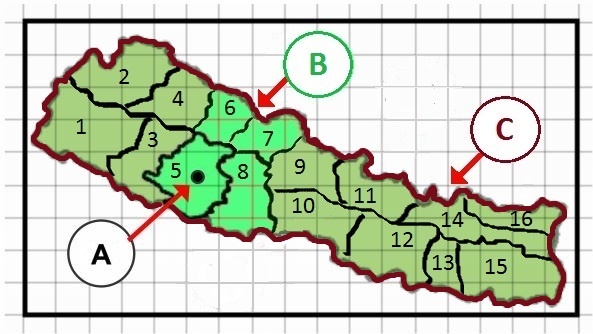
\includegraphics{nepal_ex}
\caption{Hypothetical example of spatial imprecision in aid allocation.}\label{fig:nepalex}
\end{figure}

\begin{figure}[!htbp]
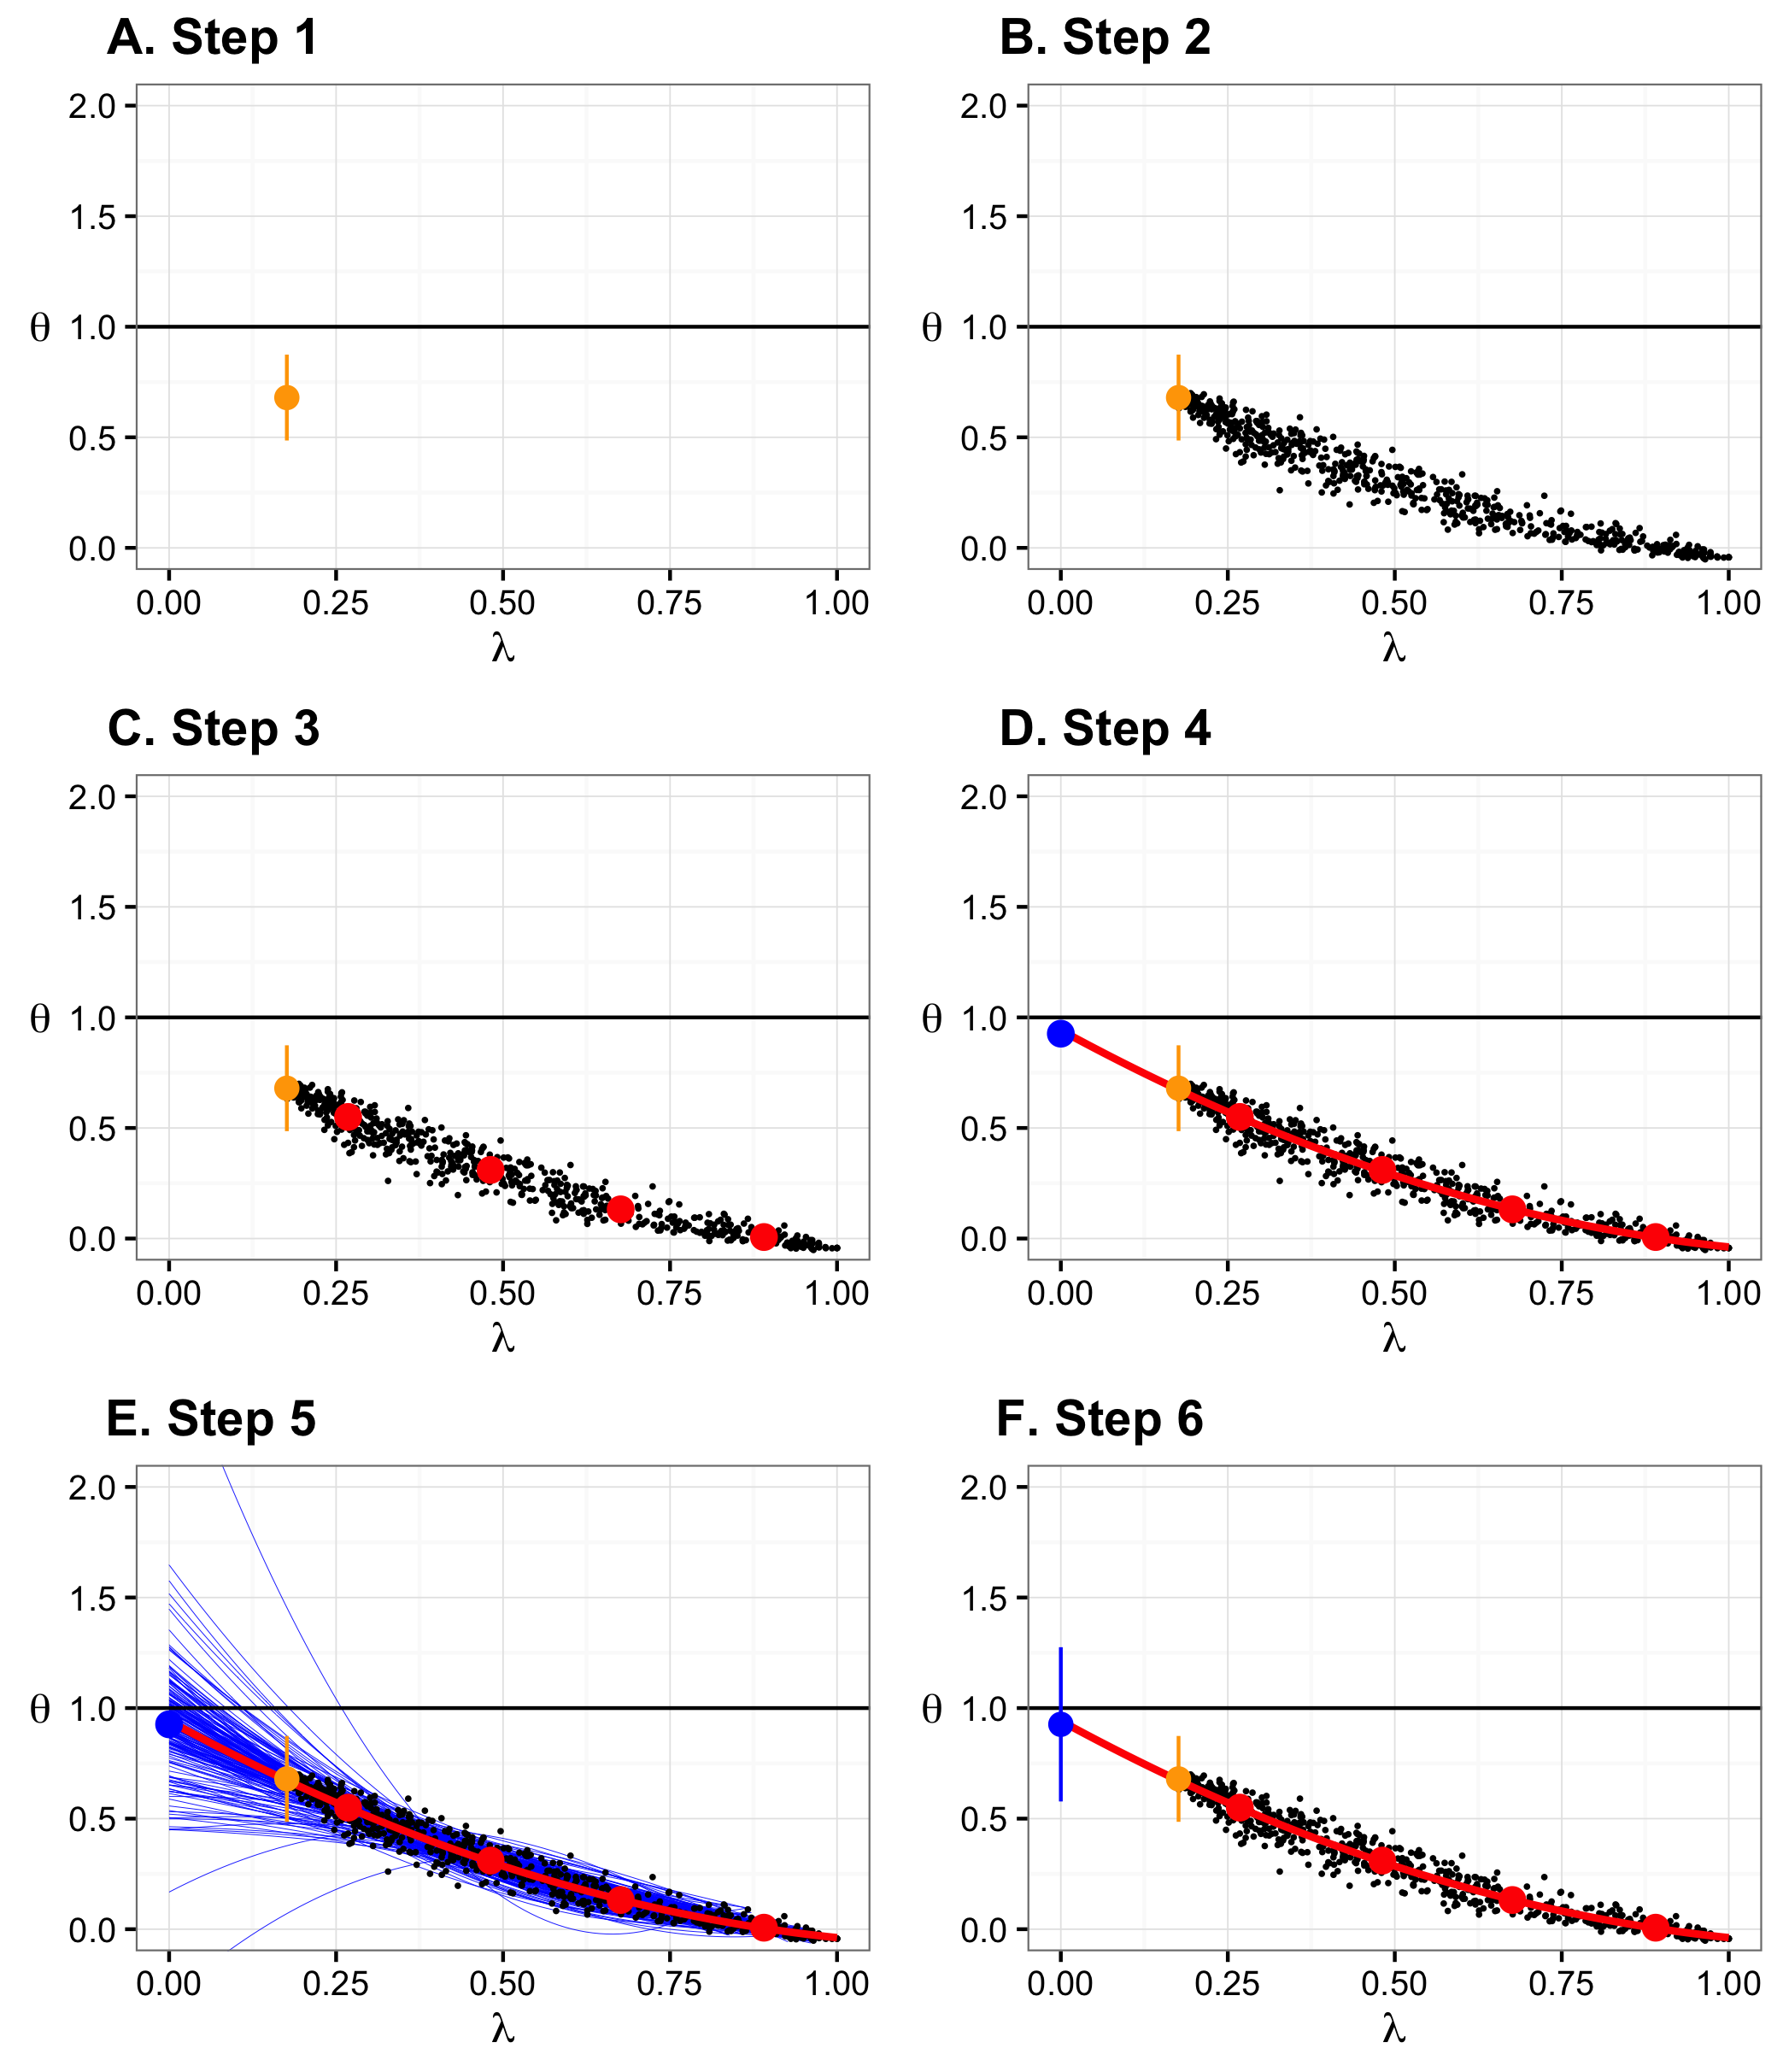
\includegraphics{steps}
\caption{Steps of the geoSIMEX procedure.}\label{fig:steps}
\end{figure}

\begin{figure}[!htbp]
\caption{Study area and units of observation.}\label{fig:studyarea}
\end{figure}

\begin{figure}[!htbp]
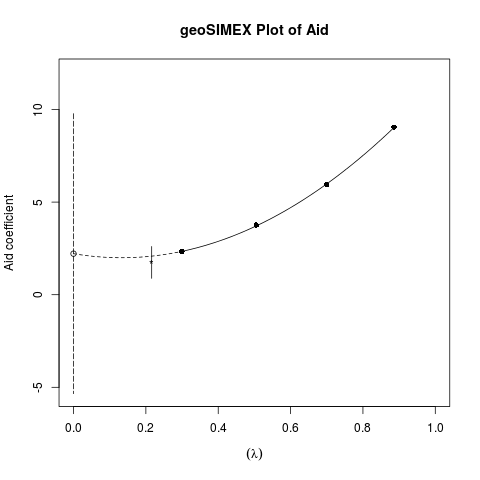
\includegraphics{geoSIMEX_plot.png}
\caption{geoSIMEX Plot of Aid.}\label{fig:geoSIMEX_plot}
\end{figure}

\newpage

%Acknowledgements
\section{Acknowledgements}
Remember: USAID grant, Relevant SciClone grants, Ben Dykstra, Ariel
\newpage

%Bibliography
\printbibliography

\end{document}
